%& -aux-directory=/tmp
% sorgt  dafuer dass aux files sonstwohin kommen -output-directory=C:/pdfout
\documentclass[10pt,a4paper, fleqn]{article}
% twocol class oder so geht auch
% fleqn macht align formeln nach lings
\usepackage[utf8]{inputenc}
\usepackage{hyperref}
\hypersetup{linktocpage}
%\usepackage[ngerman]{babel}
\usepackage{amsmath} % xrightarrow, ...
\usepackage{cite}
\usepackage{units} % nicefrac
\usepackage{datetime} % fuer Uhrzeit im \date
%\usepackage{wrapfig} % bilder rechts
\usepackage{caption} % fuer subcaption
%\usepackage{subcaption} % subfigures
\usepackage{graphicx} % Bilder allgemein einbinden
%\usepackage{tabularx} % Tabellen
\usepackage{lastpage} % Anzahl Seiten
\usepackage{multicol} % zweispaltige Titelseite
\usepackage{a4wide} % bessere Papiernutzung
\usepackage{fancyhdr} % Header/Footer
%\pagestyle{fancy} % Kopf/Fussbereich der Seiten
\usepackage{amssymb} % therefore = dreieckdots
\usepackage{array} % tables
\usepackage{booktabs} % better tables
\usepackage{floatrow} % caption beside image

% zweispaltiger Text
\usepackage{multicol}
%\setlength{\columnseprule}{0.4pt}

% Ueberschriften kleiner 	
%\usepackage{titlesec}
%\titleformat{\section}{\large\bfseries}{\thesection}{1em}{}
%\titlespacing{\paragraph}{%
%  0pt}{%              left margin
%  0.5\baselineskip}{% space before (vertical)
%  1em}%               space after (horizontal)
%%\titlespacing{\section}{0pt}{0.2\baselineskip}{0.1\baselineskip}
%\titlespacing{\align}{0pt}{0.2\baselineskip}{0.1\baselineskip}
%\titlespacing{\equation}{0pt}{0.2\baselineskip}{0.1\baselineskip}

% abgefahrenes highlighting von formeln
\usepackage{xcolor}
% klappt net, was einfacheres:
\newcommand{\highlight}[1]{%
  \colorbox{green!30}{$\displaystyle#1$}}

% Kopfzeile/Fusszeile mit fancy
%\fancyhead{}
%\fancyfoot{}
%\fancyfoot[FL]{\slshape F-Praktikum, Supraleiter}
%\fancyfoot[FR]{\slshape Page \thepage {} / \pageref*{LastPage}}
%\renewcommand{\headrulewidth}{0 pt}

% Bibliography
\bibliographystyle{ieeetr}

% Farben (werden derzeit nur in hypersetup verwendet)
\usepackage{color}
\definecolor{darkblue}{rgb}{0,0,.6}
\definecolor{darkred}{rgb}{.1,0,0}
\definecolor{darkgreen}{rgb}{0,.5,0}

% Schriften
% Palatino for rm and math | Helvetica for ss | Courier for tt
\usepackage{mathpazo} % math & rm
\linespread{1.05}        % Palatino needs more leading (space between lines)
\usepackage[scaled]{helvet} % ss
\usepackage{courier} % tt
\normalfont
\usepackage[T1]{fontenc}

% Hyperref aufsetzen
\hypersetup{
    pdftitle={Master Physik bei Nicolini, Calc writeup},
    pdfauthor={Sven Köppel},
    pdfsubject={master},
    pdfkeywords={physik} {master} {uni} {frankfurt} {fias},
    colorlinks=true,        % test: stat gerahmten Links
    linkcolor=red,          % color of internal links
    citecolor=darkgreen,    % color of links to bibliography
    filecolor=darkred,      % color of file links
    urlcolor=cyan           % color of external links
}

% Allgemeine Meta-Daten, derzeit ungenutzt
\title{\vspace{-9ex} Calc11 \vspace{-1ex}} % vertikalen platz weg...
\author{\small %
\href{https://itp.uni-frankfurt.de/~koeppel}{Sven Köppel} \\
\small \texttt{koeppel@fias.uni-frankfurt.de}}
\date{\small Generation date: \today, \currenttime}


\begin{document}
\maketitle

% abkuerzungen:
\renewcommand{\d}{\mathrm{d}}
\newcommand{\dd}[2]{\frac{\mathrm{d} #1}{\mathrm{d} #2}}
\newcommand{\pp}[2]{\frac{\partial #1}{\partial #2}}
\renewcommand{\L}{L_P}
\newcommand{\pr}{p_r}
\newcommand{\psenk}{p_\perp}
\newcommand{\ebenso}{\biggl( ~ \therefore ~ \biggr) }
\newcommand{\metrik}[1]{\d s^2 = \left( #1 \right) \d t^2 \left( #1 \right)^{-1} \d r^2 + r^2 \d \Omega_{D-2}^2 }
\newcommand{\winkel}{r^2 \d \Omega^2}
\newcommand{\dann}{$\rightarrow~$}
\newcommand{\CA}{ {\cal A}}
\newcommand{\C}[1]{ {\cal #1}}
\newcommand{\mn}{_{\mu\nu}}

\begin{multicols}{2}
This is a summary of all things I calculated or determined so far, that is, everything from the papers {\it Calc1} to {\it Calc10}, with corrections (like better graphs). It will not repeat every detailed calculation.

\columnbreak
\tableofcontents
\end{multicols}

\section{Setup}
I investigate Schwarzschild-like spherical symmetric Black Holes at short scales. The modification is expressed as a smeared Dirac mass/density term. Calculations are done with $n$ Large spatial extra dimensions in total $D=n+4$ dimensions.

Let $H(r)$ be an approximation of the Heaviside step function $\Theta(r)$, then I frequently derived the metric $g_{00}=1-V(r)$ starting from the energy density $\rho(r)$
%
\begin{equation}
\rho(r) = \frac M {\Omega_{n+2}} \dd{H(r)}r \quad\Rightarrow\quad
V(r) = \frac{2}{n+2} \frac{M}{M_*^{n+2}} {\frac{1}{\Omega_{n+2}}} \frac{H(r)}{r^{n+1}}.  \label{eq:start}
\end{equation}
%
with the surface term $\displaystyle \Omega_{n+2} = 2 \frac{\pi^\frac{n+3}{2}}{\Gamma\left(\frac{n+3}{2}\right)}$ and the reduced $d$-dimensional Planck mass $M_*$.

I examined two special choices of $H \in \{ h, h_\alpha \}$, however most relations can be derived for general (infinetly differentiable) profiles $H(r)$. These two choices each exhibit special features that will be discussed. Because $\Theta$ is dimensionless, they can be expressed in the dimensionless variable $z=r/L$ (for details see Calc9) with $H(r)=H(z)$:
%
\begin{subequations}
\begin{align}
h(r) &= \frac{r^{2+n}}{r^{2+n} + L^{2+n}} \label{eq:holo} 
&h(z) &= \frac 1{1+\left( \frac 1z \right)^{2+n}}
\\
h_\alpha(r) &= \frac{r^{3+n}}{(r^\alpha + L^\alpha/2)^{\frac{3+n}{\alpha}}} \label{eq:selfreg}
&h_\alpha(z) &= \frac{1}{\left(1+\left(\frac 1z\right)^\alpha / 2\right)^{\frac {3+n}{\alpha}}}
\end{align}
\end{subequations}
%
\newpage
The derivatives appear in many places and is therefore denoted here. Since $\dd fr = \dd fz \dd zr = \frac 1L \dd fz$, we can always substitute $H'(r) = H'(z) / L$.

\begin{subequations}
\begin{align}
h'(r) &= \frac{(2+n)~ r^{1+n} L^{2+n}}{(r^{2+n} + L^{2+n})^2}
&h'(z) &= \frac {(2+n) \left( \frac 1z \right)^{3+n}}
{\left( 1 + \left( \frac 1z \right)^{2+n} \right)^2}
= (2+n) \frac{h^2(z)}{z^{3+n}}
 \\
h'_\alpha(r) &= \frac{(n+3) L^{\alpha } r^{n+2}
   \left(\frac{L^{\alpha
   }}{2}+r^{\alpha
   }\right)^{-\frac{n+3}{\alpha
   }}}{L^{\alpha }+2 r^{\alpha
   }}
&h'_\alpha(z) &= \frac{ \frac {3+n}{2} \left( \frac 1z \right)^{\alpha+1}} {\left(1+\left(\frac 1z\right)^\alpha / 2\right)^{\frac {3+n}{\alpha} + 1}}
\end{align}
\end{subequations}

\subsection{The Mass}
We can argue that $M$ is just a constant, responsible for fulfilling the horizon equation $V(r_H)=1$. Therefore we set (»arbitrarily«)

\begin{equation}
M = \frac{n+2}{2} M_*^{n+2} \Omega_{n+2} \frac{r_H^{n+1}}{H(r_H)} 
= \frac{n+2}{2} ~\Omega_{n+2}~ \frac{1}{H(r_H)} \left( \frac{r_H}{L_*} \right)^{n+1} ~M_*
 \label{eq:M}
\end{equation}

then the horizon equation $V(r)=0$ is fulfilled at $r=r_H$. In general, equation \ref{eq:M} gives us a relationship $M=M(r)$. See Calc9, Section 1.1 for details.

\subsection{Event Horizons}
(The explicit determination of $g_00(r_H) = 0$ is straightforward and was skipped in the Calc{\it X} series until now)

\newpage
\section{Remnants}
The remnant is the smallest possible Black Hole solution and considered as a stable particle that can no more evaporate. Self encoding solutions ($h_\alpha$) encode the remnant radius by it's degrees of freedom. Typically the (reduced) Planck Length is supposed to be equal to the remnant's size. See Calc7, Section 1.1 for details. See figure \ref{fig:extremal} for a picture.

\begin{figure}[h]
%\center%
\floatbox[{\capbeside\thisfloatsetup{capbesideposition={left,top},capbesidewidth=4cm}}]{figure}[\FBwidth]
{\caption{Extremal Configuration in regularized Schwarzschild metrics. Since $g_{00}(r) \to 0$ at $r\in\{0,\infty\}$, there must be an extremal $r_0$. In the extremal configuration (blue), $r_0 = r_H$. There are also solutions with two $r_H$ and $r_0<0$ and no $r_H$, $r_0>0$. The dashed line is the Schwarzschild behaviour. See Calc7, Section 1.1 for details.}\label{fig:extremal}}
{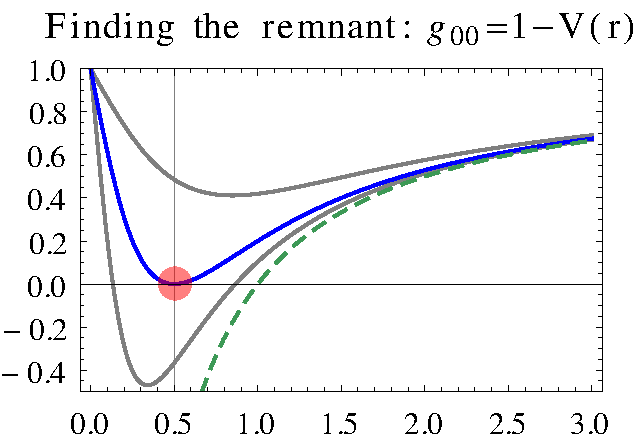
\includegraphics[width=10cm]{../Master-Calc7/mathematica/remnant-plot.pdf}}
\end{figure}

\subsection{Extremal radius and Minimal Length}
The remnant equations require
%
\begin{equation}
\begin{cases}
  \left. \partial_r \right|_{r=r_0} g_{00}(r) &= 0 \\
  g_{00}(r_0) &= 0
\end{cases}
\end{equation}
%
For our generic solution (\ref{eq:start}), we rewrite the first equation to (see Calc7 for derivation)
%
\begin{equation}
\partial_r V(r) = 0
    = -(n+1) \frac{G(r)}{r} + H'(r)
    = \left.L~H'(z)  -\frac{n+1}z~H(z)  \right|_{z=\frac{r_0} L}
\end{equation}
%
This equation can be solved for both $h(r_0)$ and $h_\alpha(r_{0,\alpha})$. In Calc7 and Calc9 I derived
%
\begin{subequations}
\begin{align}
r_0 &= L~\left( \frac 1{1+n} \right)^{\frac 1{2+n}}
 \label{eq:r0holo}\\
r_{0,\alpha} &= L~\left( \frac 1{1+n} \right)^{\frac 1\alpha}
\label{eq:r0alpha}
\end{align}
\end{subequations}

\subsection{Self-Encoding}
Self-Encoding means that $M(r_0) = M*$, so at the minimal length, the remnant has the Planck Mass. Self-Encoding only occurs in the self-regular metric, as derived in Calc7. It allows relating $\alpha = \alpha(n)$. I found that
%
\begin{equation}
\alpha_0 = \frac {3+n}{\ln(2+n)} \ln \frac {3+n}2
\end{equation}
%
\section{Thermodynamical properties}
All calculations in this section start with a generic $V(r)$, so we forget (\ref{eq:start}) for a short moment, but keep (\ref{eq:M}). That is, we have:
%
\begin{subequations}
\begin{align}
V(r) &\equiv M(r_H) \cdot Y(r) \label{eq:simpleV} \\
M(r_H) &\equiv Y^{-1}(r_H)% \quad\quad\leftarrow\text{this does }\textbf{not}\text{ say } M=Y^{-1}
\label{eq:simpleM}
\end{align}
\end{subequations}
%
The smearing solution (\ref{eq:Y}) reconstructs equation (\ref{eq:start}), with an appropriate dimensionful constant~$A$:
%
\begin{subequations}
\begin{align}
Y(r) &= A \frac{H}{r^{n+1}} \label{eq:Y} \\
V(r) &= A~M(r_H)~\frac{H(r)}{r^{n+1}} \\
M(r_H) &= \frac{1}{A} \frac{r_H^{n+1}}{H(r_H)}
\end{align}
\end{subequations}
%
\subsection{Hawking Temperature}
Let's start with a generic $V(r)$ from which we don't know the inner structure yet:
%
\begin{align}
T &\equiv \frac{1}{4\pi} \left. \partial_r g_{00} \right|_{r=r_H}
= - \frac{1}{4\pi} M(r_H) \cdot Y'(r_H)
= - \frac{1}{4\pi}\frac 1L M(z_H) Y'(z_H) 
\end{align}
%
Details can be found in Calc9, Section 1.6. With the holographic approach these equations read
%
\begin{align}
T &= \frac{1}{4\pi r_H} \left( 1 + n - r_H \frac{H'(r_H)}{H(r_H)} \right)
 = \frac 1L \frac{1}{4\pi z_H} \left( 1 + n - z_H \frac{H'(z_H)}{H(z_H)} \right)
 \label{eq:simpleT}
\end{align}
%
Now is simple to insert our $H\in\{h,h_\alpha\}$. Figure (\ref{fig:th}) shows $T_H$ for both of them.

\begin{figure}[h]
\center%
% makebox laesst uebergrosses Bild mittig werden
\makebox[\textwidth][c]{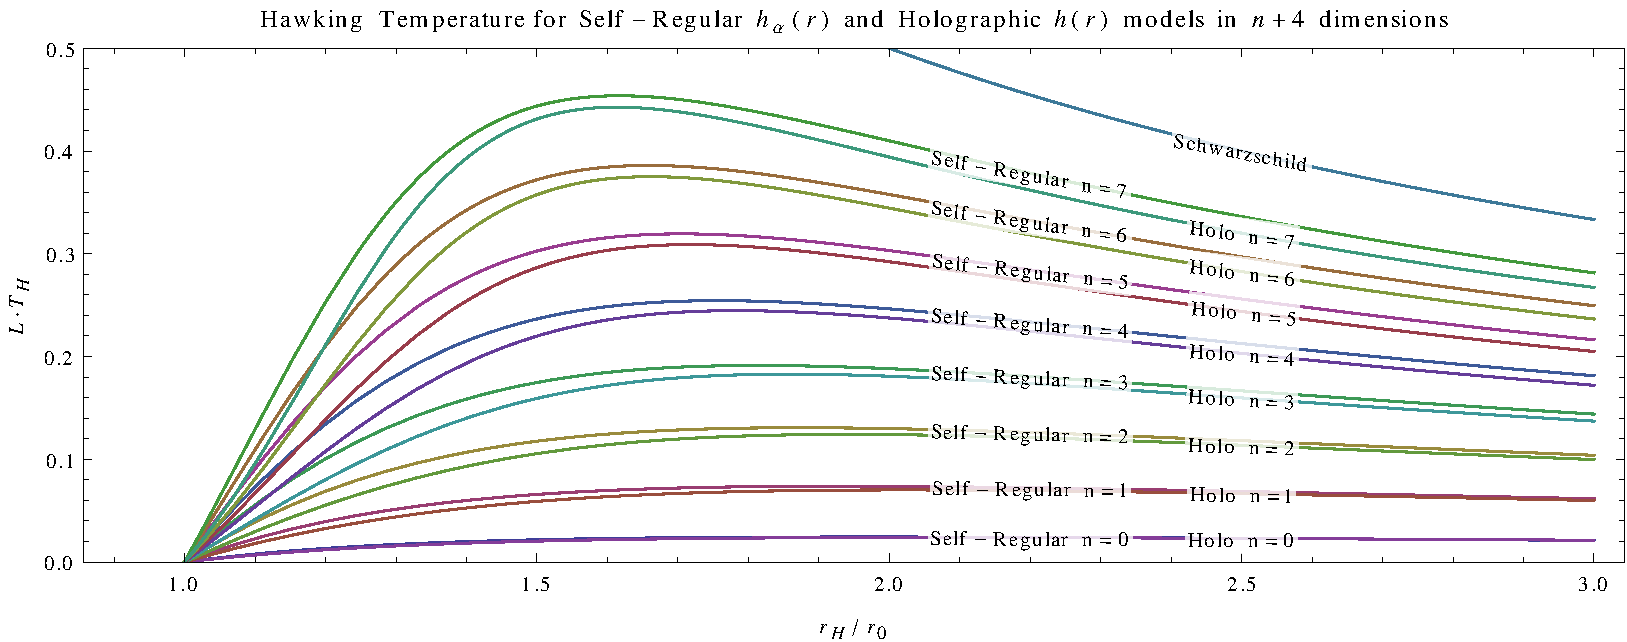
\includegraphics[width=1.3\textwidth]{mathematica/thawking.pdf}}
\caption{Hawking temperature for the holographic model $h$ and the Self-Regular mode $h_\alpha$. The functions are $L \cdot T_H(r_H/r_0)$. The Schwarzschild-Tangherlini solution is shown for comparison.
}\label{fig:th}
\end{figure}

\newpage
\subsection{Heat Capacity}
The determiniation of the Heat Capacity is done by variable substitution:
%
\begin{equation}
C = \pp{M}{T_H} = \pp{M}{r_H}\left(\pp{T_H}{r_H}\right)^{-1} \label{eq:C}
= \pp{M}{z_H} \left(\pp{T_H}{z_H}\right)^{-1}
\end{equation}
%
Inserting (\ref{eq:M}) and (\ref{eq:simpleT}), we get
%
\begin{equation}
C = 
\frac{4\pi r_H^{n+2}}{A}
\frac{r_H H'\left(r_H\right)-(n+1) H\left(r_H\right)}
   {r_H^2 H\left(r_H\right)
   H''\left(r_H\right)-r_H^2 H'\left(r_H\right){}^2+(n+1) H\left(r_H\right){}^2}
\end{equation}
%
Especially $C(r) = L^n~C(z)$.

At the critical radius $r_C$ a phase transition takes place. It is $C(r_C) = 0$ and $T_H(r_C)$ is extremal (so $\left. \partial_{r_H} T_H \right|_{r_H=r_C}=0$). The critical radius for $h(r_C)$ and $h(r_{C,\alpha})$ is given by

\begin{align}
r_C & = 2^{\frac{1}{n+2}} \left(-n^2+(n+2) \sqrt{n^2+2 n+5}-3 n-4\right)^{-\frac{1}{n+2}} \\
r_{C,\alpha} &= \textit{no closed expression for general n, but possible for fixed n}
\end{align}

Figure \ref{fig:heat1} shows the well-known curve. In figure \ref{fig:heat0} the abscissa is rescaled by $r_C$, so $(r_H-r_C)r_0$ is displayed (numerical evaluation of $r_C$ for convenience).

\begin{figure}
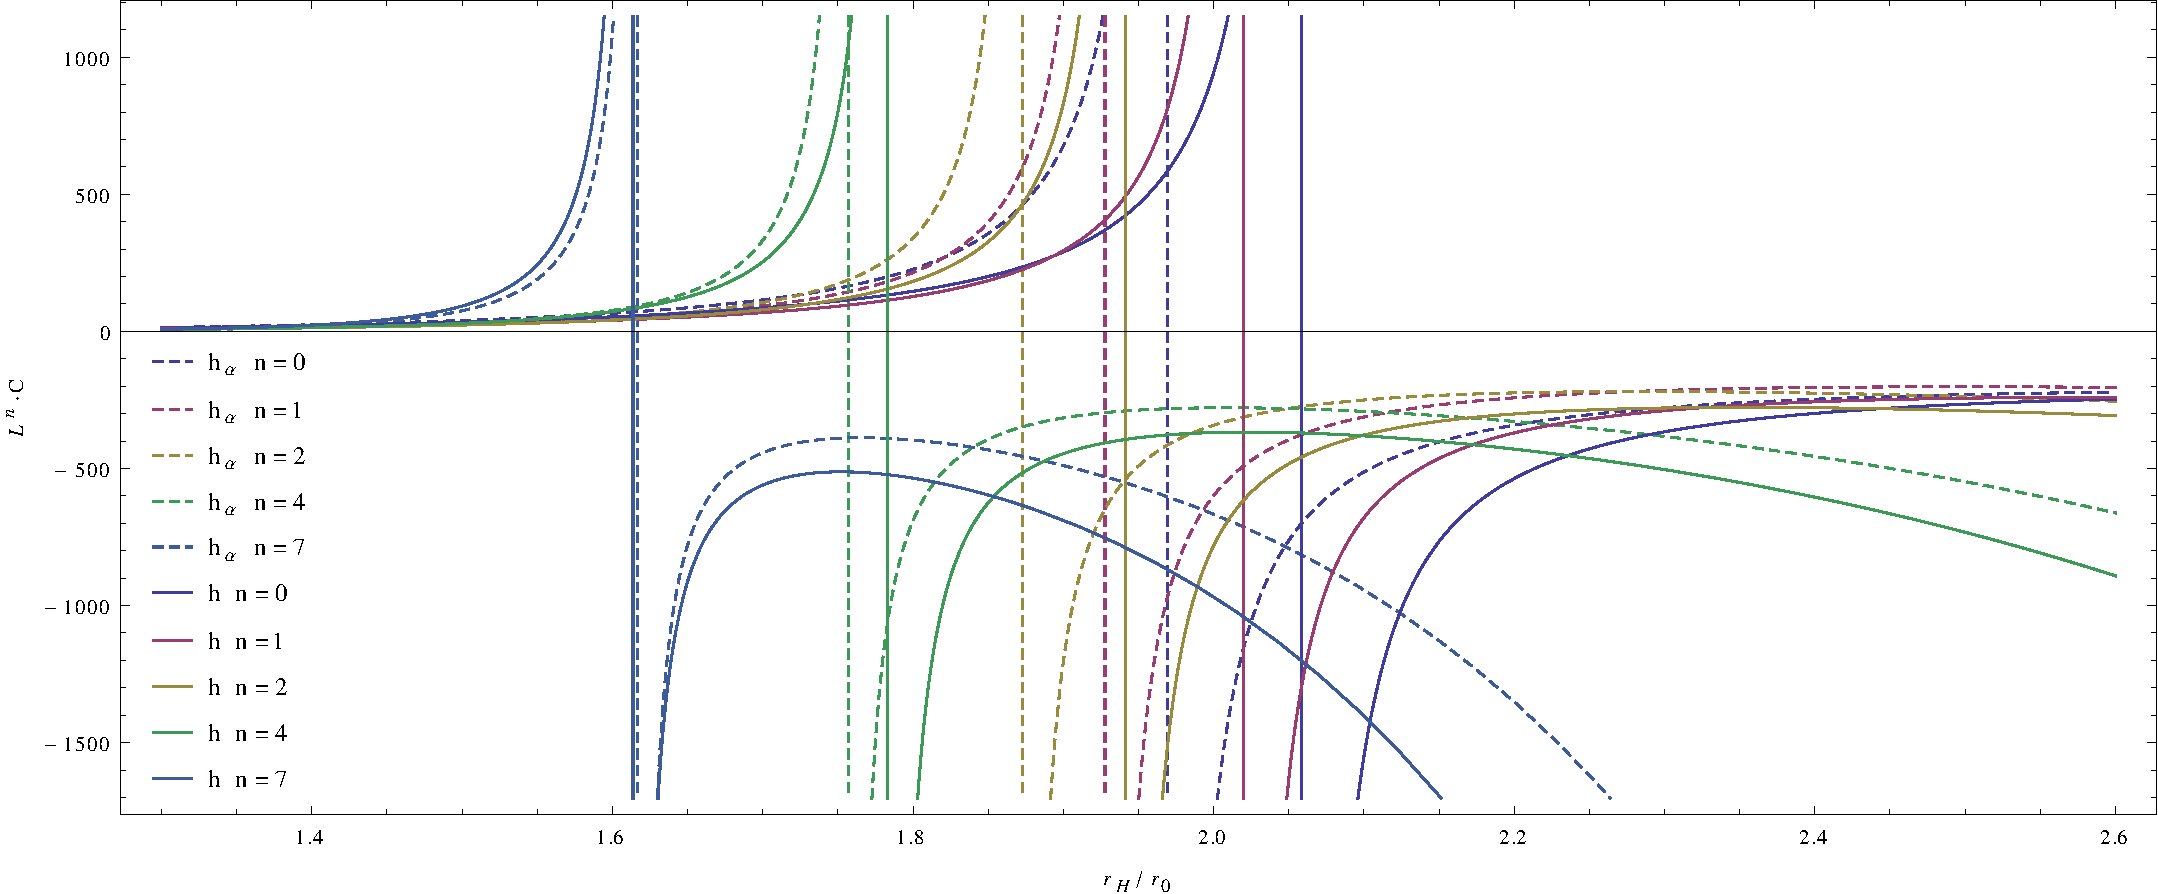
\includegraphics[width=\textwidth]{mathematica/th-holo-nicer.pdf}
\caption{Heat Capacity for $h(r)$ and $h_\alpha(r)$ in various dimensions with critical $z_C$ clearly visible (c.f. figure \ref{fig:th}). Figure \ref{fig:heat0} shows the same functions shifted with $r_C$} \label{fig:heat1}
\end{figure}

\begin{figure}
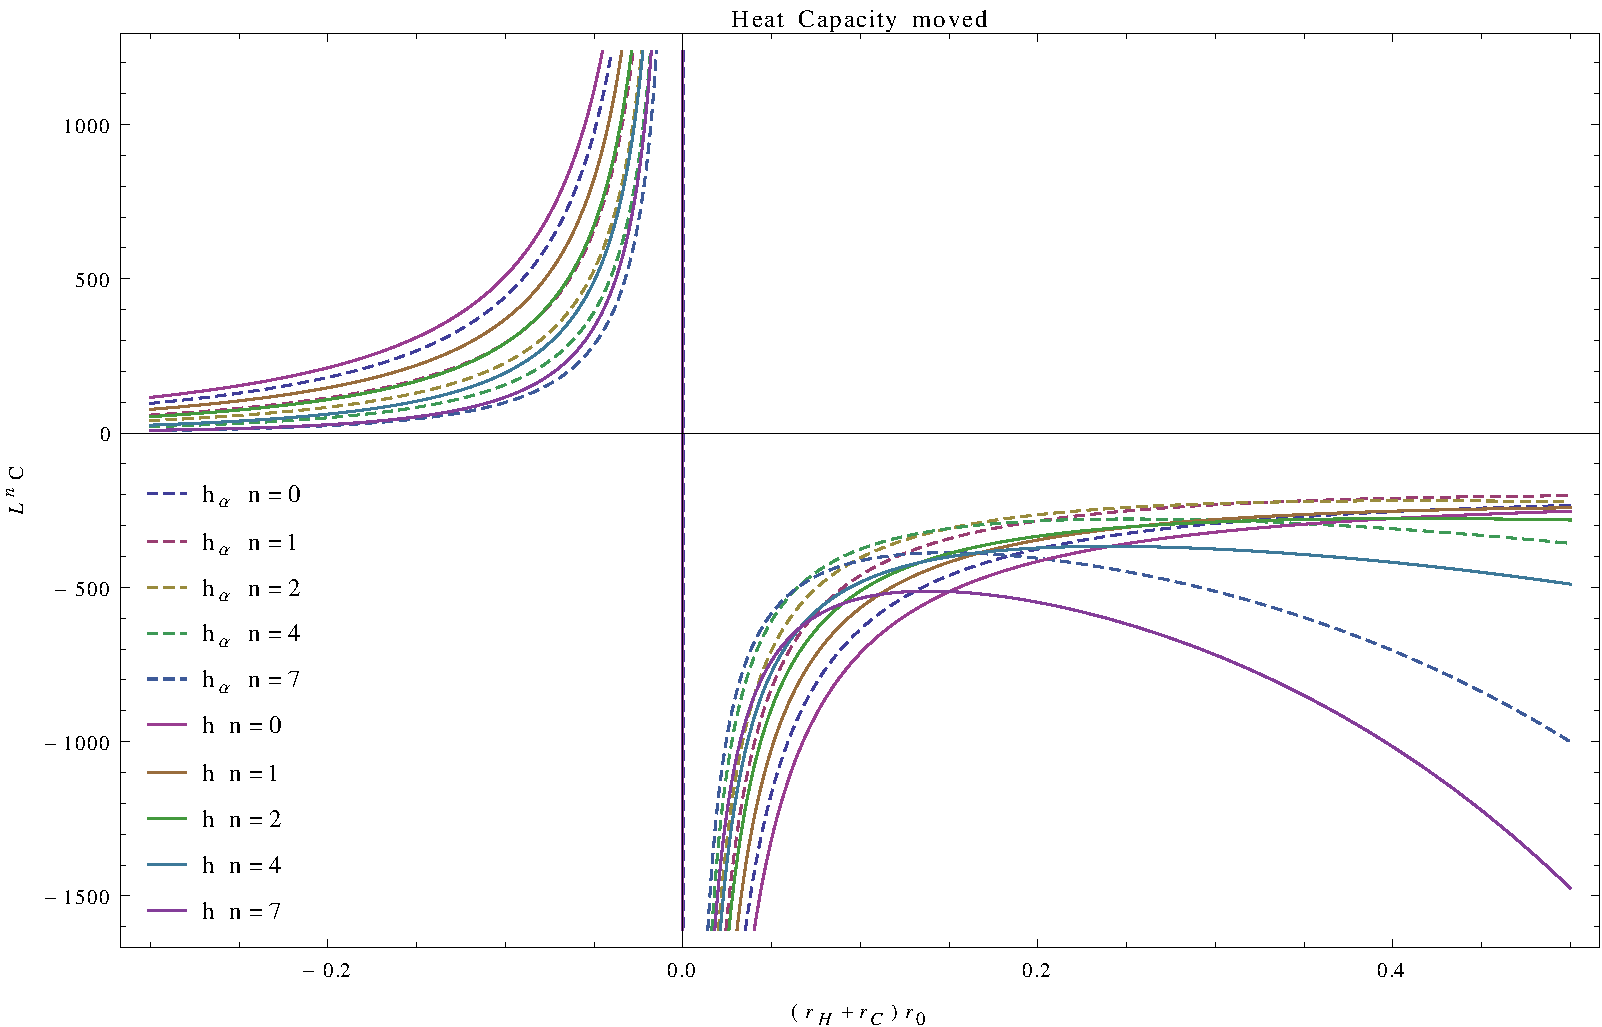
\includegraphics[width=0.9\textwidth]{mathematica/heat-capacity-rC.pdf}
\caption{Heat Capacity shifted around $r_C$ (c.f. figure \ref{fig:heat1})}\label{fig:heat0}
\end{figure}

\subsection{Entropy}
%Entropic corrections are interesting for the hologrpahic model.
%
The entropy defining integral can also be subsituted like in the Heat Capacity in the section before:
%
\begin{subequations}
\begin{align}
S(r) &= \int^{M_2}_{M_1} \frac{\d M}T = \int_{r_1}^{r_2} \dd M{r_H} \frac {\d r_H}T = \int \d r_H \frac 1T \left( \dd{M(r_H)}{r_H} \right) \\
S(z) &= \int \d z_H \frac 1T \left( \dd{M(z_H)}{z_H} \right)
=  -4\pi L \int^z \d z_H\frac{M'(z_H)}{M(z_H)} \frac  1{Y'(z_H)} 
\end{align}
\end{subequations}
%
Inserting (\ref{eq:M}) and (\ref{eq:simpleT}) yields (I label $z_H=x$)
%
\begin{subequations}
\begin{align}
S(z) &= -4\pi L \int^z \d x \left( \frac {n+1}x - \frac {H'(x)}{H(x)} \right) \frac 1{Y'(x)} \\
&= -4 \pi LA \int^z \d x \left( \frac {n+1}x - \frac {H'(x)}{H(x)} \right)
\frac{x^{n+2}}{x H'(x) - (n+1) H(x)}  \label{eq:Sgeneric} 
\end{align}
\end{subequations}
%
This integral can be computed, at least for the hologrpahic model $h(r)$. This allows us to see logarithmic corrections in any dimension:
%
\begin{equation}
S_h(z) = 4\pi A L \left( \frac{x^{n+2}}{n+2} + \log(x) \right)^z_1
\end{equation}
%
See Calc9 Section 1.6.3 for details.

\newpage
\section{Modified Einstein Equations}
It is reasonable to find a deeper concept to justify the smearing of the Schwarzschild source. This can be smearing the Ricci scalar with a bilocal distribution $\C A^2(x-y) = \C A^2(\square_x) \delta^D(x-y)$ and was done in Calc8 and Calc10.

Based on the density (\ref{eq:start}), one tries to find $\C A$:
%
\begin{equation}
\C T^0_0 = -M \CA^{-2}(\square) \delta(\vec x)
\stackrel{!}{=} - \frac M{\Omega_{n+2}} \dd{H(r)}r  \label{eq:TA}
\end{equation}
%
A Fourier transform helps to find the solution for the operator (for Details see Calc10, Section 1.1)
%
\begin{equation}
\CA^{-2}(p^2) = \C F \left\{ \dd{H(x)}x \right\}
= \int_{-\infty}^\infty \d^{3+n} r~\dd{H(r)}r~e^{-ipr}
\end{equation}
%
For $h(r)$, I found the Meijer G-function as a closed algebraic solution, 
%
\begin{equation}
p~\C A^{-2}(p) \propto G_{p,q}^{\,m,n} \left( \left. \begin{matrix} a_1, \dots, a_p \\ b_1, \dots, b_q \end{matrix}\; \right| \; z \right)
\end{equation}
%
The $p$-dependence enters into the $z$ part while the lists are only $l$ and $n$-dependent.


\end{document}